\section{$^{24}$Mg}
In the following section, results for $^{24}$Mg are presented, it's a natural choice to study how well deformations are represented by our framework, since it's light, very deformed and shows no pairing interaction in its ground state.
\subsection{\texttt{HFBTHO} code and calculation details}
\subsubsection{\texttt{HFBTHO}}
To benchmark the code in the case of nuclear deformation, the \texttt{HFBTHO} code was used \cite{MAREVIC2022108367}, it's a HFB code which minimizes the energy functional on a (Transformed) Harmonic Oscillator basis. Since $^{24}$Mg is a light nucleus, it still works well in this case.
\\All calculations are carried out using a number of shells of $12$ and a null pairing interaction. Default paramters for the quadrupole constraints were used.
\subsubsection{Code parameters and axial constraint}
As for our code, calculations are performed on a box $[-10, 10]$ fm.
In the case of the ground state calculation, a step size of $0.33$ fm is used, with a starting guess of a deformed Woods-Saxon with $\beta_2=0.4$.
\\The calculation in the case of the deformation curve is carried out imposing the following constraints
\begin{align}
  \expval{\Re\mathcal Q_{22}} = 0
  \\\expval{\Im \mathcal Q_{22}} = 0
  \\\expval{\mathcal Q_{20}} = q_{20}.
\end{align}
These constraints altogether impose an axial deformation on the system. This is done because on a full mesh like in our case, the nucleus may deform on a different axis from the chosen one (z), resulting in spurious contributions to the real deformation curve; moreover, the axial symmetry of $\texttt{HFBTHO}$ doesn't allow broken axial symmetry configurations.
\\Regarding the stiffness $c$ and damping parameter $\mu$ of ALM \ref{sec:alm}, $c=0.001$ and $\mu=0.1$ were used. As for convergence criteria, a tolerance of $0.001$ on the value of $\beta_2 - \beta_{2, \text{target}}$ was used.
\subsubsection{Ground state}
Table \ref{tab:mg_table} reports data for the ground state of $^{24}$Mg, compare with $\texttt{HFBTHO}$ results, while figure \ref{fig:mg_gs_density_axial} shows the total particle density.
Charge radii for the two codes are displayed but not compared, due to different formulas used for their computation.
\begin{table}[ht]
  \centering
  \begin{tabular}{lrrccc}
    \addlinespace[0.3em]
    \toprule
    && GCG & \texttt{HFBTHO} & $\Delta$ & $\Delta\%$ \\
    \midrule
    $E_{\text{TOT}}$& [MeV]    & -195.854 &-197.030 & 1.176 & 0.597 \\
    $\expval{ r^2_n}^{1/2}$    &[fm] & 3.0124    & 2.9996 & 0.0128  & 0.427\\
    $\expval{ r^2_p}^{1/2}$    &[fm] & 3.0475    & 3.0326  & 0.0149 & 0.491\\
    $\expval{ r^2_{ch}}^{1/2}$ &[fm] & 3.5390    & 3.4614  & - & - \\
    $\expval{z^2}^{1/2}$ &[fm] & 2.1454 &-  &- &-\\
    $\expval{x^2}^{1/2}$ &[fm] & 1.5112 &- & -&-\\
    $\expval{y^2}^{1/2}$ &[fm] & 1.5147 &- & -&-\\
    $\beta_2$ &[-] & 0.399 &0.390 & 0.009 & 2.3  \\
    \bottomrule
  \end{tabular}
  \caption{Results for $^{24}$Mg ground state, no pairing interaction, box $[-10, 10]$ fm, step size 0.33 fm, SKM* parametrization.}
  \label{tab:mg_table}
\end{table}
\begin{figure}[h]
  \centering
  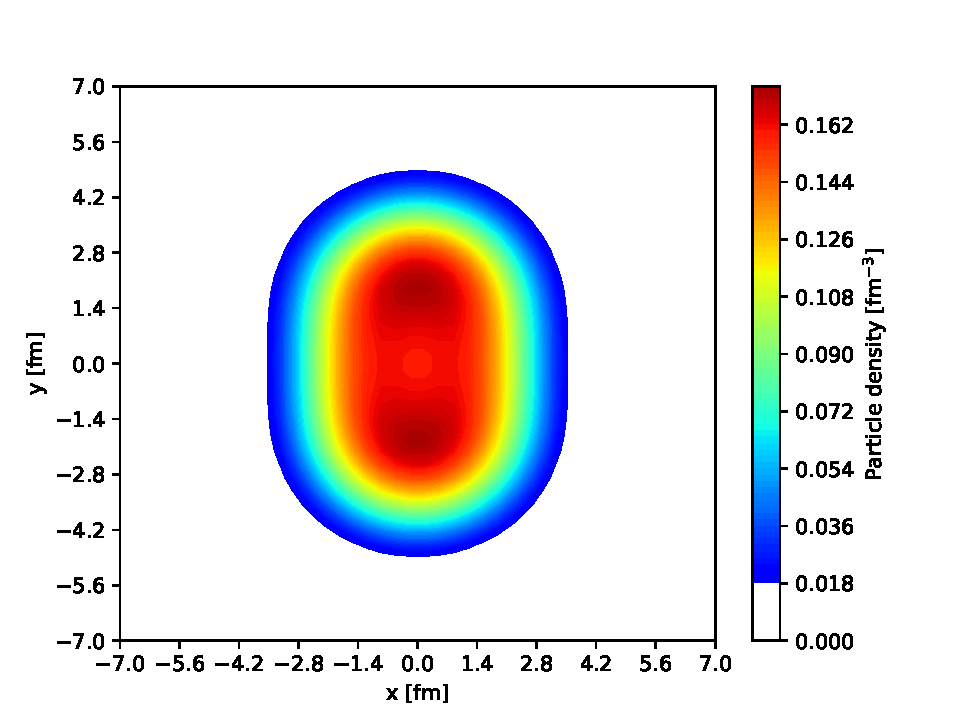
\includegraphics[width=1.0\linewidth]{Images/mg_gs_density_axial.pdf}
  \caption{Magnesium ground state density, calculation done on a box $[-10, 10]$ fm, step size 0.33 fm, SKM* parametrization}
  \label{fig:mg_gs_density_axial}
\end{figure}
\subsubsection{Deformation curve}
In figure \ref{fig:mg_no_pair_deformation}, the deformation curve is shown for $^{24}$Mg, without pairing. To counteract the sharp rise in CPU time, due to the high number of points in the curve, a coarser grid is used, hence the different minimum energy and $\beta_2$ values than the ones reported in table \ref{tab:mg_table}.
\begin{figure}[h]
  \centering
  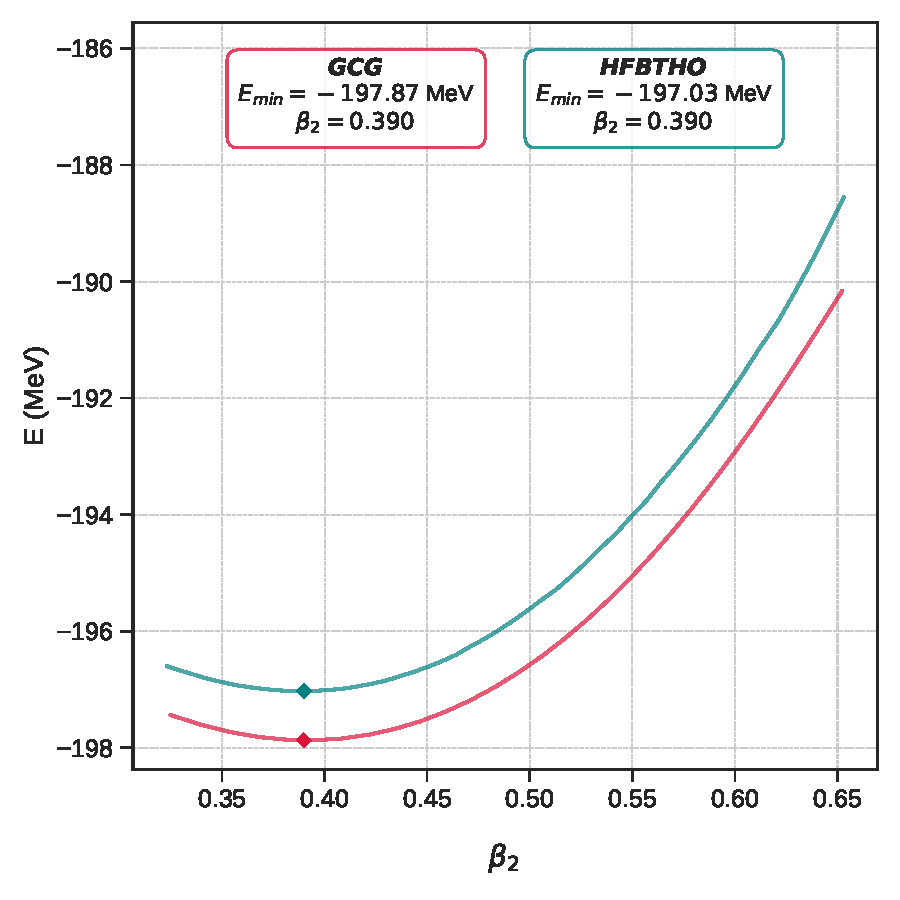
\includegraphics[width=0.8\linewidth]{Images/mg_nopair_curve.pdf}
  \caption{Magnesium deformation curve, no pairing interaction, calculation done on a box $[-10, 10]$ fm, step size 0.66 fm, SKM* parametrization.}
  \label{fig:mg_no_pair_deformation}
\end{figure}